\documentclass[12pt]{article}

\usepackage{amsmath}
\usepackage[authoryear,round]{natbib}
\usepackage{hyperref}



\textwidth=6.2in
\textheight=8.5in
\oddsidemargin=.1in
\evensidemargin=.1in
\headheight=-.3in

\newcommand{\scscst}{\scriptscriptstyle}
\newcommand{\scst}{\scriptstyle}
\newcommand{\Rfunction}[1]{{\texttt{#1()}}}
\newcommand{\Rmethod}[1]{{\texttt{#1}}}  
\newcommand{\Rclass}[1]{{\texttt{#1}}}
\newcommand{\Robject}[1]{{\texttt{#1}}}
\newcommand{\Rpackage}[1]{{\textit{#1}}}
\newcommand{\code}[1]{{\texttt{#1}}}
\bibliographystyle{plainnat}

\title{Outline: Analysis of High Throughput Flow Cytometry Data using \Rpackage{plateCore}}

%%%%%%%%%%%%%%%%%%%%%%%%%%%%%%%%%%%%%%%%%%%%%%%%%%%%%%%%%%%%%%%%%%%%%%%%%%%
\usepackage{C:/R/R-2.7.0rc/share/texmf/Sweave}
\begin{document}
\maketitle

\tableofcontents

%%%%%%%%%%%%%%%%%%%%%%%%%%%%%%%%%%%%%%%%%%%%%%%%%%%%%%%%%%%%%%%%%%%%%%%%%%%%%%%%%%%%%%%%%%%%%%%%%%%%%%%%%%%%%%%%%%%%%%%%%%%%%%%%%%%
\section{Abstract}
\Rpackage{plateCore} is a Bioconductor packaged created to make processing and analysis of large, complex flow datasets
in R easier. High throughput flow studies are often run in a 96 or 384-well plate format, with a number of different samples, 
controls, and antibodies-dye conjugates present on the plate. Analyzing the output from the cytometer requires keeping track of the contents
of each well, matching sample wells with control wells, gating each well/channel separately, making the appropriate plots, quality assessment, and
summarizing the results. \Rpackage{plateCore} extends the \Rpackage{flowCore} and \Rpackage{flowViz} packages to work on
\Rclass{flowPlate} objects that represent these large flow datasets. For those familiar with \Rpackage{flowCore} and \Rpackage{flowViz}, 
the gating (filtering), transformation, and other data manipulations for \Rclass{flowPlates} are very similar to \Rclass{flowSets}. 

In this document we show how use \Rpackage{plateCore} to analyze a publicly available blood dataset. This peripheral blood
mononucleocyte (PBMC) data was generated using BD FACS\texttrademark CAP screening to look at the expression profiles of 189 
different antibodies. The raw PBMC data is read into R using \Rpackage{flowCore}, and then the filtering and 
threshold gating are performed in \Rpackage{plateCore}. The output is the fraction of positive (expressing) cells for
each marker.

%%%%%%%%%%%%%%%%%%%%%%%%%%%%%%%%%%%%%%%%%%%%%%%%%%%%%%%%%%%%%%%%%%%%%%%%%%%%%%%%%%%%%%%%%%%%%%%%%%%%%%%%%%%%%%%%%%%%%%%%%%%%%%%%%%
\section{Introduction}
Analysis of flow cytometry high content screening (FC-HCS) experiments requires a systematic approach to
preprocessing, gating (i.e., filtering), and summarizing large amounts of data. Ideally these steps would be automated,
allowing analysis pipelines to be robust, objective, and match the high-throughput capacity of modern cytometers. 
Unfortunately, current approaches to FC-HCS analysis methods are semi-automated at best,
often requiring significant manual intervention to identify cells of interest and set the appropriate gates. 
Since the manual contribution is subjective and prone to error when working with large numbers of samples, it
is desirable to develop programmatic approaches to process the data.

Flow cytometry packages available through the Bioconductor project provide an open analysis platform that
can be used by cytometrists, bioinformaticians, and statisticians to develop new analysis approaches that
enable automated processing. The \Rpackage{flowCore} package contains the framework for importing, transforming, gating, and
organizing raw flow cytometry data. \Rpackage{flowViz} supports sophisticated visualizations based on Trellis displays. 
\Rpackage{flowClust} implements model-based clustering approaches for automated gating. The combination of
these packages provides a set of freely available, flexible, and computationally efficient FC-HCS tools.

\Rpackage{plateCore} provides a convenient way to manage the sample annotation associated with complex FC-HCS experiments, and
to access the functionality in other Bioconductor flow packages. Since the layout of FC-HCS plates often changes from experiment
to experiment, the annotation for each well needs to be customized for each \Rclass{flowPlate}. \Rpackage{plateCore}
uses an approach that is very similar to the cell-based high throughput screening \Rpackage{cellHTS2} package,
where users must provide a \textit{plate configuration} file for each dataset. Once the cell level data has
been analyzed in \Rpackage{plateCore}, the summary well information (i.e., percentage of positive cells and median
signal intensities) can be imported into tools like \Rpackage{cellHTS2}, since FC-HCS experiments are just one 
type of cell-based high throughput screens.

The progression from raw FCM data files to a completed \Rpackage{plateCore} analysis is shown in Figure~\ref{fig:analysis}.


\begin{figure}
\centering
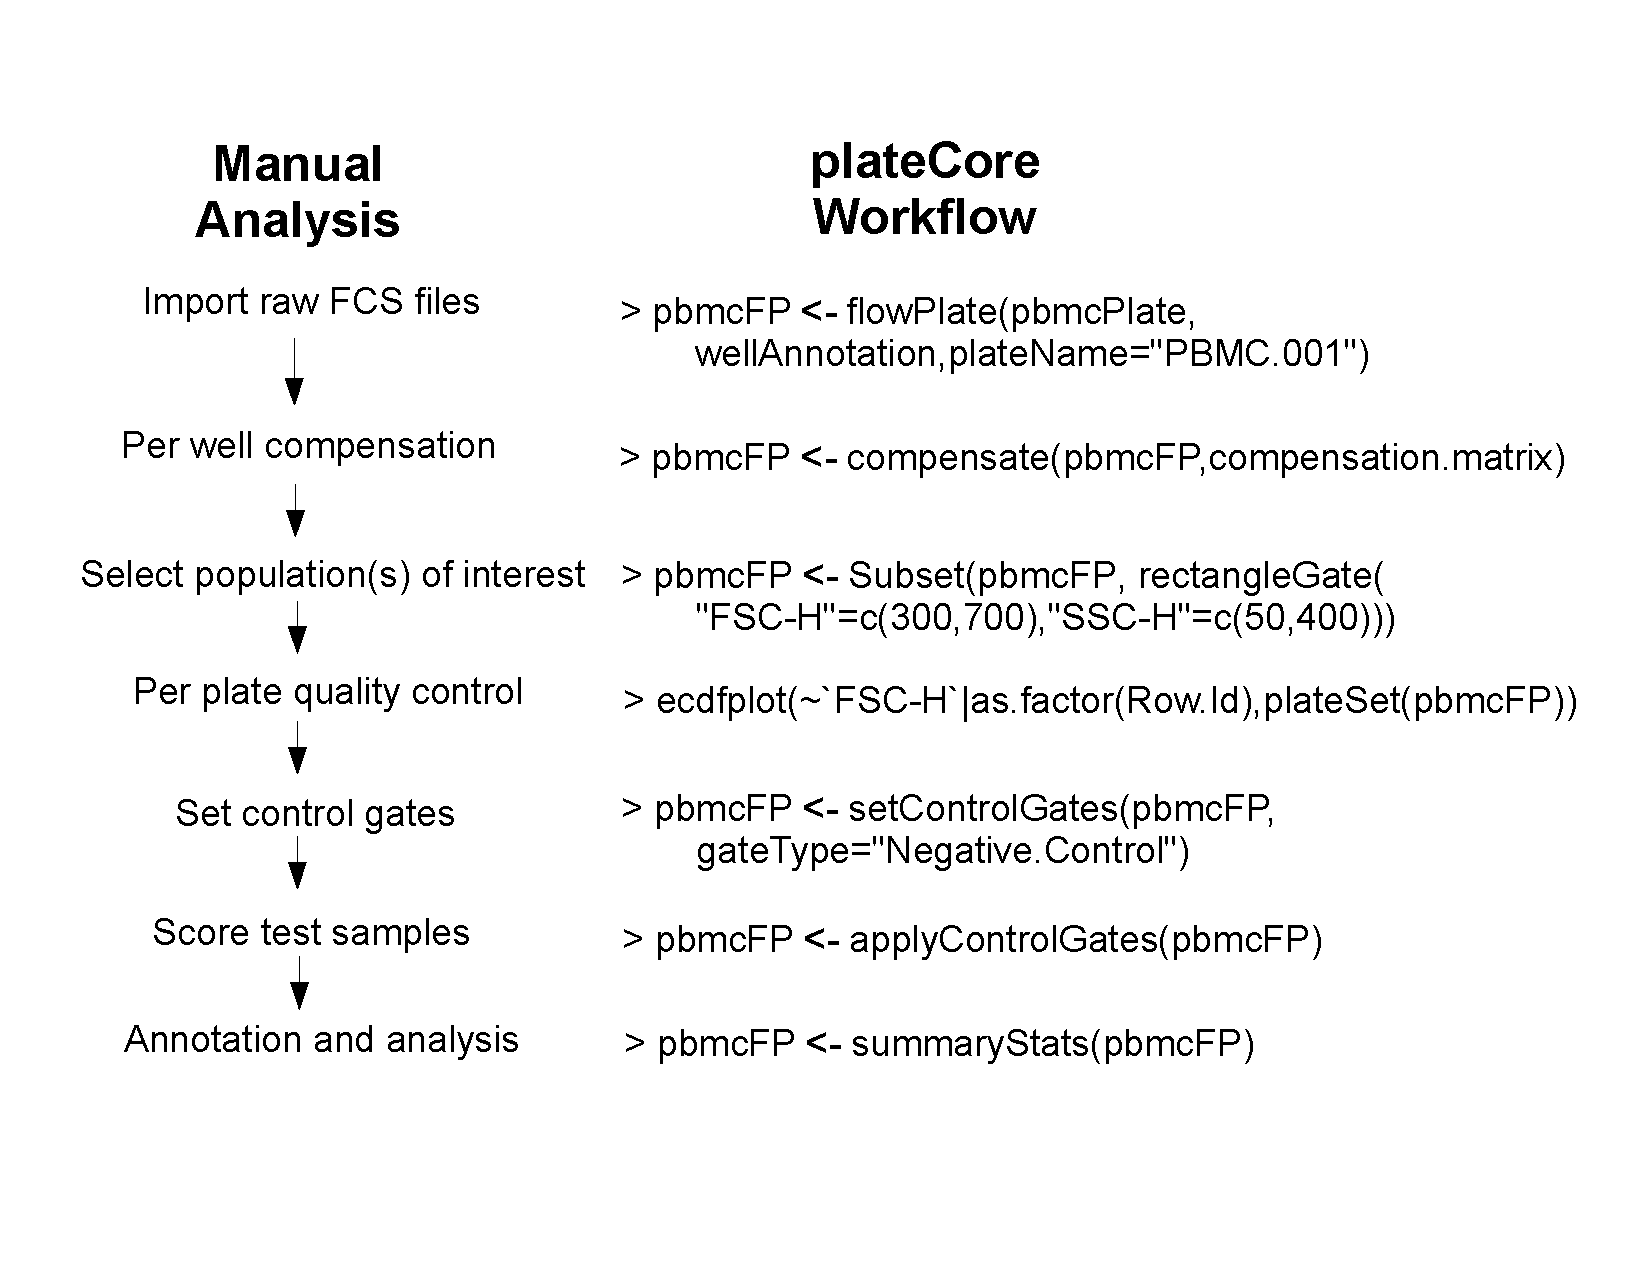
\includegraphics{analysisSteps.pdf}
\caption{Typical plateCore analysis on the left, and examples of each step from a sample analysis are shown on the right.
Performing quality assessments and generating reports are multi-step actions and the code required is not shown here.
If necessary, the threshold control gates created automatically from setControlGates are adjusted based on input from flow experts. 
These new gates are established based on the gap between negative control wells and positive test samples, whereas the automated
control gates were set using only negative control wells.}
\label{fig:analysis}
\end{figure}
 
%%%%%%%%%%%%%%%%%%%%%%%%%%%%%%%%%%%%%%%%%%%%%%%%%%%%%%%%%%%%%%%%%%%%%%%%%%%%%%%%%%%%%%%%%%%%%%%%%%%%%%%%%%%%%%%%%%%%%%%%%%%%%%%%%%%
\clearpage
\section{Example Data}
The PBMC dataset used in this example is available for download from ficcs.org as the "plateData.tar.gz" file. The data consists
of 5 different peripheral blood mononucleocyte (PBMC) samples that were analyzed with 189 different antibodies on 96-well plates. Each plate has a set of
unstained, isotype, and control wells. Antibodies and isotype controls are arrayed 3 per well, and the data was compensated
on the cytometer. The \textit{plate configuration} is also included in the archive as \textit{maskPlateDesc.csv} (Note: I need
to update the description so it's compatible with the latest version of plateCore).
Unfortunately, the antibody names have been masked since the layout of the plate is proprietary. (Although
I'm cautiously optimistic that we will be able to release more information about the experiment).

%%%%%%%%%%%%%%%%%%%%%%%%%%%%%%%%%%%%%%%%%%%%%%%%%%%%%%%%%%%%%%%%%%%%%%%%%%%%%%%%%%%%%%%%%%%%%%%%%%%%%%%%%%%%%%%%%%%%%%%%%%%%%%%%%%%
\section{Analysis}
FCS files for each plate are imported in R using \Rpackage{flowCore}, and a \Robject{flowPlate} named platePBMCraw is created by integrating
the \textit{plate configuration} with the \Robject{flowSet}. The data in this experiment has already been compensated on
the cytometer, so there is no need to correct for spillover in R. This analysis will focus on lymphoctyes, which
will be selected using a rectangular forward (FSC) and side-scatter (SSC) morphology gate (Figure ~\ref{fig:morphGate}).

\begin{Schunk}
\begin{Sinput}
> platePBMC <- Subset(platePBMCraw, rectangleGate("FSC-H"=c(300,700),"SSC-H"=c(50,400)))	
\end{Sinput}
\end{Schunk}

Wells that are affected by fluidic events, which can cause a temporary shift in the cytometer detector readings, need
to be identified and either corrected or removed from the analysis. The \Rfunction{qaProcess.timeline} from
the \Rpackage{flowQ} package can be used to search for fluidic events in \Rclass{flowSets} by looking for shifts in specific channels that
are above some predetermined threshold. Fluidic events can also often be identified by plotting the median FSC-SSC
values for each well, and looking for values that are outside the central population (Figure ~\ref{fig:fluidic}).



\begin{figure}
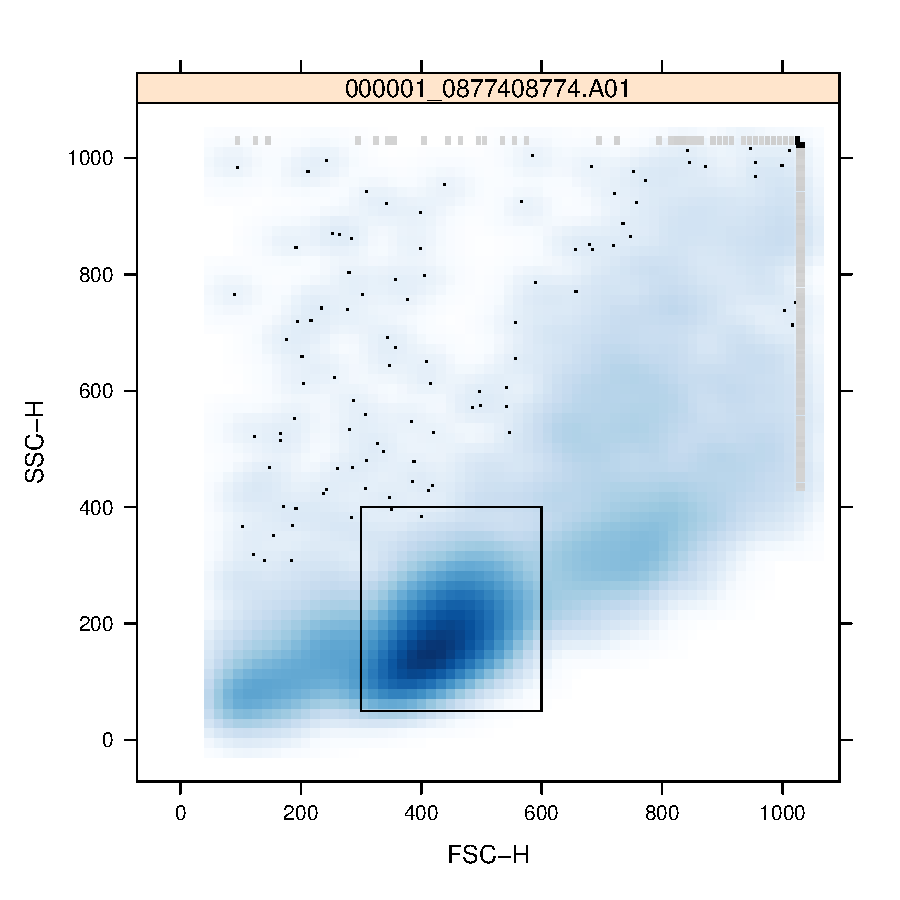
\includegraphics{outline-morphGate}
\caption{rectangleGate used to select lymphocytes from PBMC data.}
\label{fig:morphGate}
\end{figure}

\begin{figure}
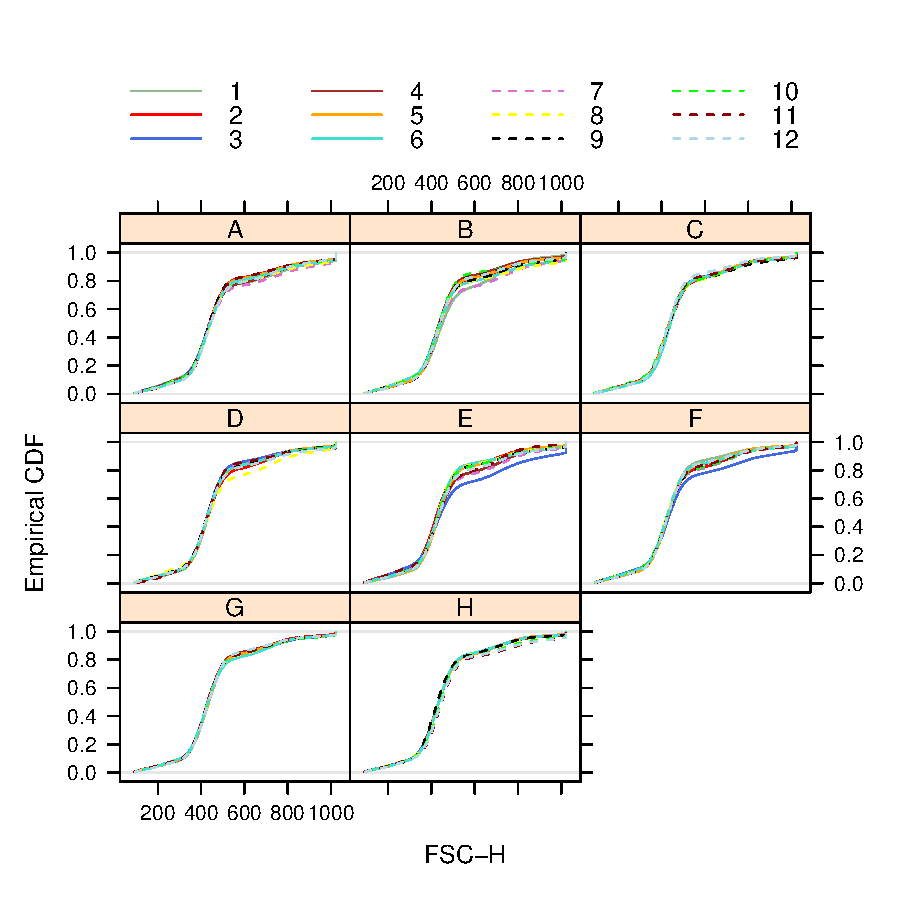
\includegraphics{outline-fluidic}
\caption{Plot of median FSC versus median SSC for one sample PBMC plate used as a quick graphical check
for wells with fluidic events. Wells in the lower right corner (H10-H12) are unstained, while
the rest of the wells were stained in 3 channels. No significant fluidic events were detected in the 
5 PBMC plates analyzed for this study.}
\label{fig:fluidic}
\end{figure}

\clearpage
Once the lymphocytes have selected using the FSC-SSC morphology gate, and the plate has passed quality control
checks, the next step is setting the control gate to establish the cutoff between positive and negative cells.
Ideally this expression threshold would be established by finding the gap known positive and negative samples, but such information is
usually not available. Instead, the expression cutoff is generally set according to some type of negative control. 
\Rpackage{plateCore} supports creating thresholds according to either unstained, unstimulated, isotype, 
or fluorescence minus one (FMO) controls. One-dimensional expression thresholds are initially set using
the setControlGates function. 
\begin{Schunk}
\begin{Sinput}
> platePBMC <- setControlGates(platePBMC,gateType="Negative.Control",numMads=6)
\end{Sinput}
\end{Schunk}
The "numMads" parameter sets the value of the control gate at 6 median absolute deviations (MADs) above 
the media fluorescence intensity (MFI) the control gate. \Rpackage{flowCore} and \Rpackage{flowClust} potentially offer
more robust methods of establishing this threshold using kernel density approaches, but setting the
gate at 3 to 6 MADs on linear scale signals often works well in practice for screening quality experiments.

Once the Negative.Control gates have been created and applied, we can then use the \Rfunction{summaryStats} to calculate different
metrics of interest from the \Rclass{flowPlate}. Running \Rfunction{applyControlGates} and \Rfunction{summaryStats} on the \Robject{platePBMC}, 
\begin{Schunk}
\begin{Sinput}
> platePBMC <- applyControlGates(platePBMC)
> platePBMC <- summaryStats(platePBMC)
\end{Sinput}
\end{Schunk}
will result in additional columns created in the associated \Robject{wellAnnotation} object associated with this
particular \Robject{flowPlate}.  
These new columns include percentage of cells above the Negative.Control gate (Percent.Positive),
the number of cells in the raw data (Total.Events), the number of positive cells (Positive Count),
the median fluorescence intensity (MFI), and the ratio of the test well MFI to the MFI of the negative
control well (MFI.Ratio). In this PMBC example a number of the samples are heterogeneous, so the MFI and MFI.Ratio
may not be helpful since they are based on all the cells in a well, and not just the positive cells.

\begin{figure}
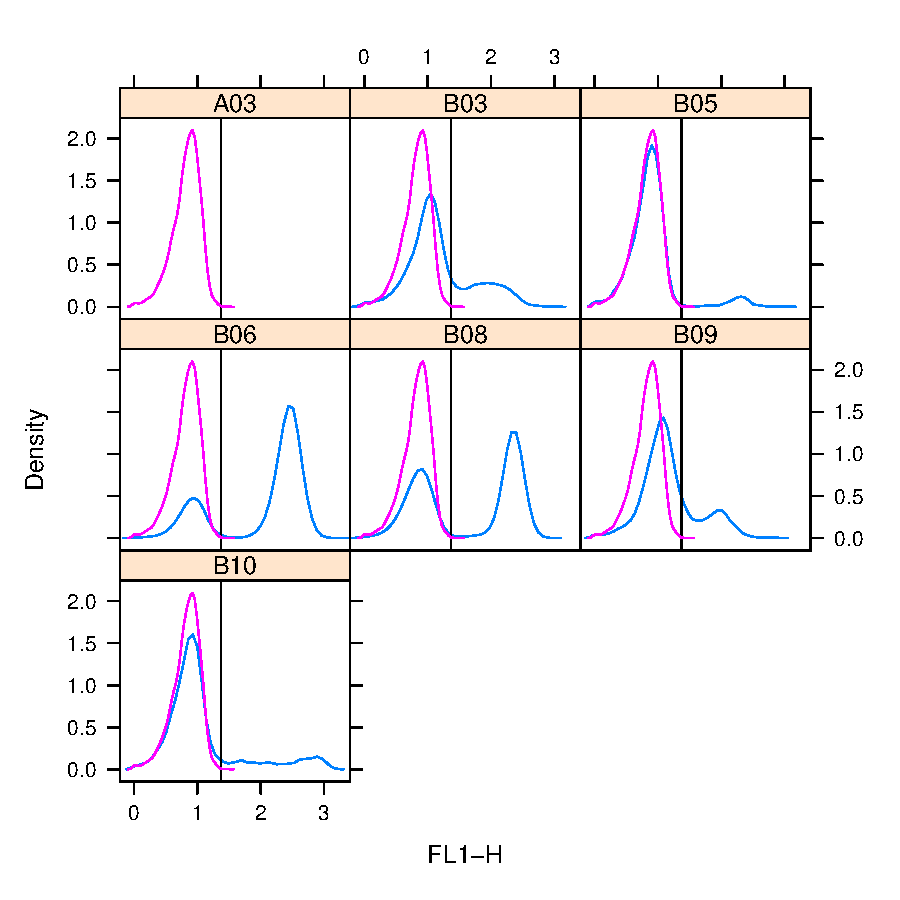
\includegraphics{outline-isoGate}
\caption{Density plots for one isotype and the associated test wells. Isotype results are shown in magenta while the test samples
are in blue. The vertical bar indicates the negative control gate, estimated using the setControlGates function with numMads=6.}
\label{fig:isoGate}
\end{figure}

\clearpage
The wellAnnotation \Robject{data.frame} associated with each analyzed \Robject{flowPlate} can then be exported from R for
use in other programs. The first few rows from the PBMC plate analyzed in this analysis are shown below.

\begin{Schunk}
\begin{Sinput}
> head(wellAnnotation(platePBMC))
\end{Sinput}
\begin{Soutput}
  Well.Id Sample.Type Ab.Name Channel Negative.Control plateName           name
1     A01     Isotype Isotype   FL1-H              A01  PBMC.001 0877408774.A01
2     A01     Isotype Isotype   FL2-H              A01  PBMC.001 0877408774.A01
3     A01     Isotype Isotype   FL4-H              A01  PBMC.001 0877408774.A01
4     A02     Isotype Isotype   FL1-H              A02  PBMC.001 0877408774.A02
5     A02     Isotype Isotype   FL2-H              A02  PBMC.001 0877408774.A02
6     A02     Isotype Isotype   FL4-H              A02  PBMC.001 0877408774.A02
  Negative.Control.Gate Percent.Positive Total.Count Positive.Count       MFI
1              23.27180       0.11612716        6889              8  7.054802
2              51.36569       0.97256496        6889             67 11.785791
3              61.62651       0.13064305        6889              9 13.984600
4              23.40704       0.05425936        7372              4  7.118605
5              24.22585       0.17634292        7372             13  6.163591
6              64.22498       0.06782420        7372              5 14.497407
  MFI.Ratio
1         1
2         1
3         1
4         1
5         1
6         1
\end{Soutput}
\end{Schunk}




%%%%%%%%%%%%%%%%%%%%%%%%%%%%%%%%%%%%%%%%%%%%%%%%%%%%%%%%%%%%%%%%%%%%%%%%%%%%%%%%%%%%%%%%%%%%%%%%%%%%%%%%%%%%%%%%%%%%%%%%%%%%%%%%%%%
\clearpage
\section{Results}

Each of the 5 PBMC data plates was analyzed using the approach described in the analysis section.  The \Robject{wellAnnotations}
for each plate was exported and merged, and the results for 83 markers with greater than 10\% positive cells are shown in Figure~\ref{fig:pbmcHeat}.
Histograms for one of the markers showing variable levels of expression between the different plates are shown in Figure~\ref{fig:pbmcCDbd69}. 
These histograms were created by binding selected wells from each plate into a virtual plate and then using
the densityplot function.
\begin{Schunk}
\begin{Sinput}
> densityplot(~ `FL2-H` | as.factor(plateName), virtPlate,filterResult="Negative.Control")
\end{Sinput}
\end{Schunk}

\begin{figure}
\begin{center}
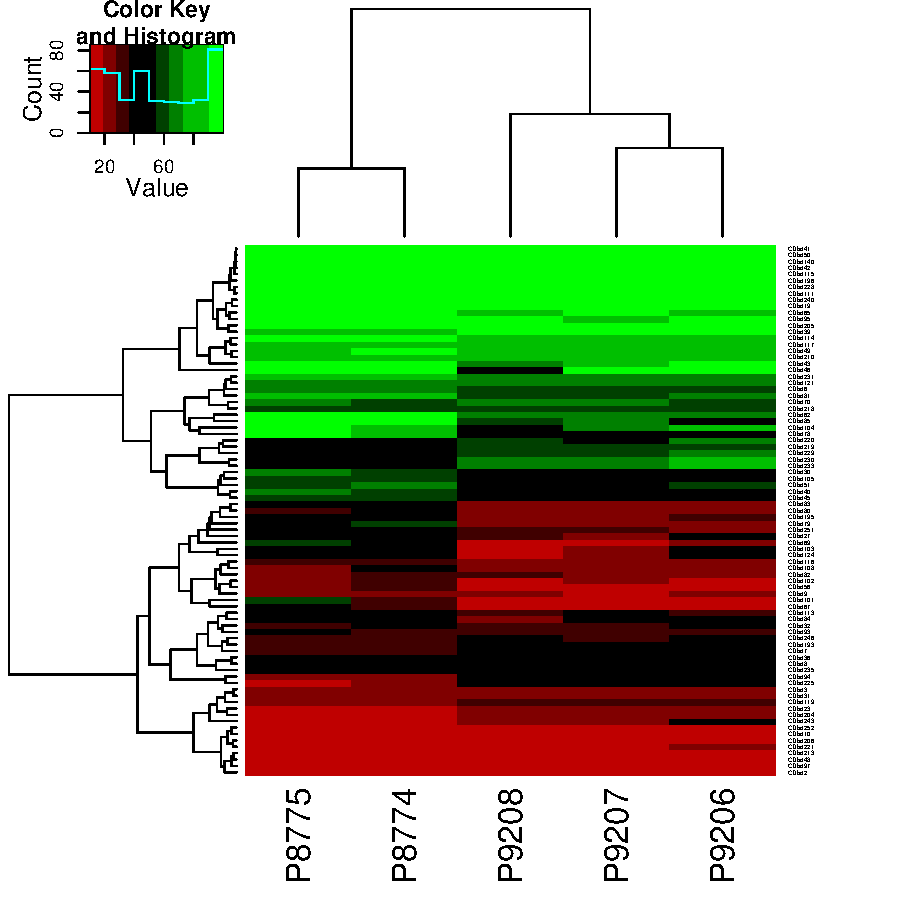
\includegraphics{outline-pbmcHeat}
\end{center}
\caption{Heatmap showing the percentage of positive cells for the 5 different PBMC lymphocyte plates.}
\label{fig:pbmcHeat}
\end{figure}

\begin{figure}
\begin{center}
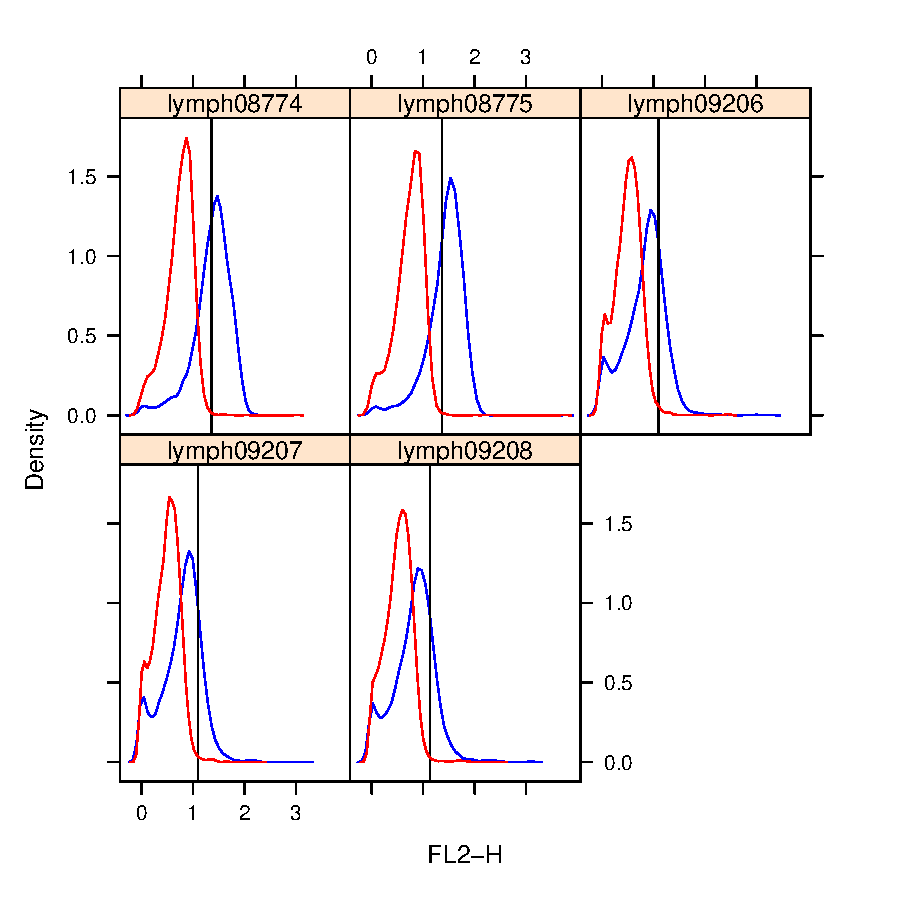
\includegraphics{outline-pbmcCDbd69}
\end{center}
\caption{Dotplots for CDbd69, which is differentially expressed between the 5 PBMC plates. Isotypes are shown in black and
test wells are in magenta.}
\label{fig:pbmcCDbd69}
\end{figure}


%%%%%%%%%%%%%%%%%%%%%%%%%%%%%%%%%%%%%%%%%%%%%%%%%%%%%%%%%%%%%%%%%%%%%%%%%%%%%%%%%%%%%%%%%%%%%%%%%%%%%%%%%%%%%%%%%%%%%%%%%%%%%%%%%%%
\clearpage
\section{Conclusions}

The PBMC example shows that a complex analysis of a 96-well plate, stained with 189 antibodies,
can be constructed in 15-20 lines of code using \Rpackage{plateCore}. Lymphocytes were selected
using \Rpackage{flowCore} gates and visualized using \Rpackage{flowViz} plots. One-dimensional 
gates were constructed using isotype wells and applied to the test wells to identify positive cells.

Given a \textit{plate configuration} file, this same approach can be used to analyze any
negative control based FC-HCS study. Although adjustments to the automatically generated negative control gates may be needed,
these changes change be incorporated into the analysis script and reproduced at a later time.

(Need some additional paragraphs about why plateCore is wonderful).

%%%%%%%%%%%%%%%%%%%%%%%%%%%%%%%%%%%%%%%%%%%%%%%%%%%%%%%%%%%%%%%%%%%%%%%%%%%%%%%%%%%%%%%%%%%%%%%%%%%%%%%%%%%%%%%%%%%%%%%%%%%%%%%%%%%
\section{References/Recent Related Publications}
\begin{itemize}
\item flowCore manuscript in Cytometry A\\
Gives an overview of flowCore data structures, transformation and gating examples, quality control checks (flowQ), and 
flowCore analysis philosophy.\\
\item Using flowViz to Visualize Flow Cytometry Data, Bioinformatics\\
Uses flowViz to make xyplots, ecdfplots, and time plots of GvHD data. Makes the case that visualizations can be used to aid automation.
\item Quality Assessment of Ungated Flow Cytometry data in High Throughput experiments, Cytometry A, GvHD data\\
Visualizing data: xyplots, histograms, ecdfplots, boxplots, and contour plots.\\
Outlier detection (Grubbs and KS)\\
Using flowViz/Core graphical output for quality assessment\\
\item Analysis of flow cytometry data using an automatic processing tool, Cytometry Part A\\
Automated analysis in Matlab.\\
\end{itemize}

\end{document}
